\documentclass[11pt,oneside,a4paper,numbers=enddot]{report} % scrreprt
\usepackage{thema}

\begin{document}
\Pre

\chapter{Inleiding}
*Fill with content*

\chapter{Weekopdracht 1}

Wij verbinden bedrijven
Wij laten bedrijven samenwerken
Community van bedrijven
Wij introduceren bedrijven aan elkaar
Matchmaker voor bedrijfrelaties
Om bedrijven makkelijk met elkaar in contact te brengen voor het delen van services.
door middel van delen van services

\section{Servicemarkt}

\subsection{Missie}
Wij zijn de marktplaats voor services
fdsjfdskfsdfksdhfjsdajfhadsfhsdajfhjasdfhjasdf

\subsection{Visie}
Wij geven bedrijven de kans om elkaar te ontmoeten zodat ze elkaar kunnen helpen. \\
Wij laten hen in contact komen zodat ze elkaars services kunnen benutten.

\subsection{Doelen}

\begin{itemize}
\item
  Wij streven ernaar om bekend te worden als
  een betrouwbare plaats om services aan te bieden
\item
  Een mooie website opzetten waar bedrijven makkelijk van kunnen maken
\item
  Koffiemachine (Oftewel goed met onze werknemers omgaan)
\item
  Wij willen het kortste lijntje tussen bedrijven zijn.
\end{itemize}

\include{txt/2}
\chapter{Opdracht week 4}

\section{Toepassing 1}

Als eerste werd er natuurlijk gedacht aan het originele idee,
een website waarop services gedeeld en ingehuurd worden.

\subsection{Relatie SWOT}
{\bf Hoe zijn we op dit idee gekomen, hoe is dit gerelateerd}

\subsection{Uitbreidingsplan}

\subsubsection{Doel}
{\bf Bedoeling met het systeem, welke partijen hebben er mee te maken}

\subsubsection{Impact}
{\bf Wat is er nodig, wat gebeurt er met het bedrijf}

Hieronder is een simpel voorbeeld van de onderliggende architectuur.

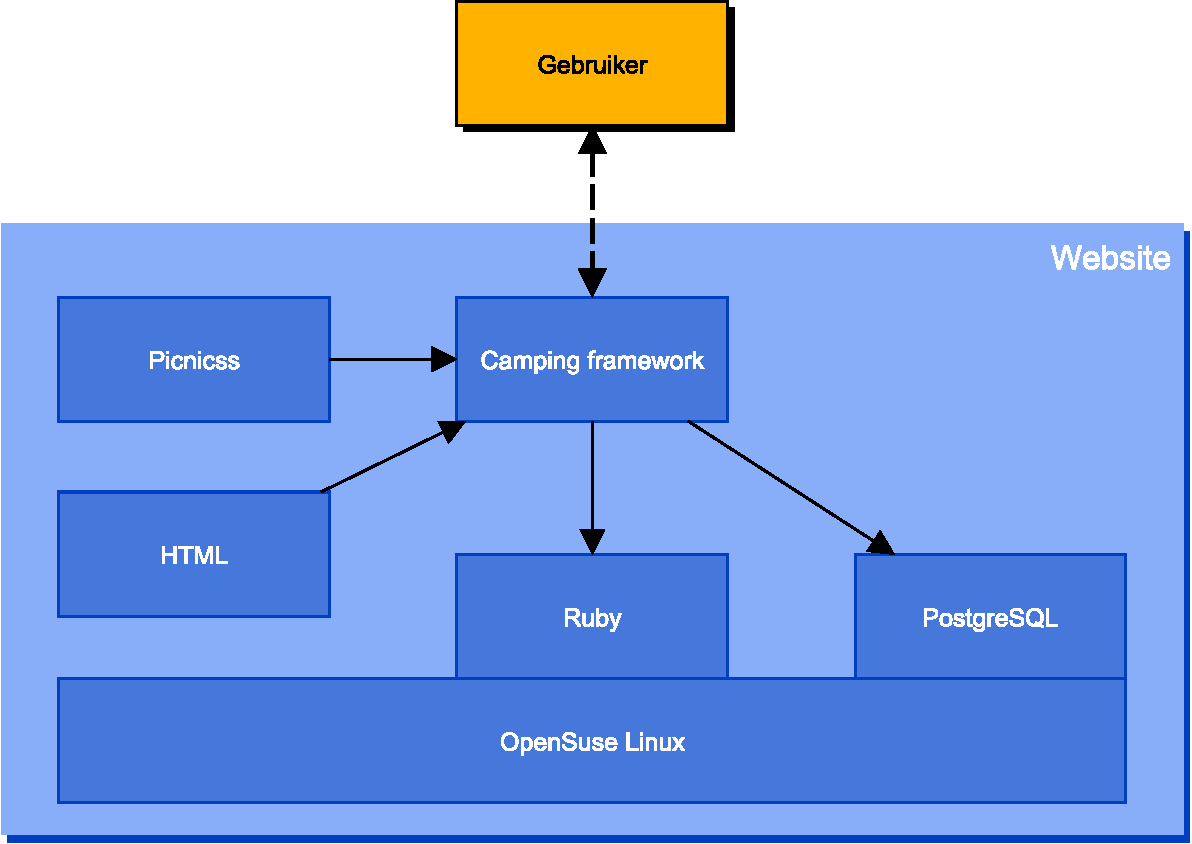
\includegraphics[width=\textwidth]{img/websiteArchitecture}

\subsubsection{Omschrijving}
{\bf Systeemontwerpen, wireframes, designs}

\section{Toepassing 2}

Een app zou eenzelfde soort functie kunnen leveren,
maar zal andere mensen aantrekken.
Een hypothese zou kunnen zijn dat een app het gemak verhoogd
en dus de markt groter maakt,
met een breder scala aan mensen.

\subsection{Relatie SWOT}
{\bf Hoe zijn we op dit idee gekomen, hoe is dit gerelateerd}

\subsection{Uitbreidingsplan}

\subsubsection{Doel}
{\bf Bedoeling met het systeem, welke partijen hebben er mee te maken}

\subsubsection{Impact}
{\bf Wat is er nodig, wat gebeurt er met het bedrijf}

\subsubsection{Omschrijving}
{\bf Systeemontwerpen, wireframes, designs}

\section{Toepassing 3}

Gezien we een handjevol competente ICT Beheerders in de groep hebben,
is het normaal om de benodigde ICT-gerelateerde services zelf te beheren.
Omdat er een grote kans is dat er meerdere servers benodigd zullen zijn,
is het belangrijk om een goede basis te hebben.

\subsection{Relatie SWOT}
{\bf Hoe zijn we op dit idee gekomen, hoe is dit gerelateerd}

Het bedrijf is gefocused op snelle communicatie,
hiervoor is een stabiel platform erg belangrijk.
Dit systeem zorgt er ook voor dat systeembeheerders meer 'agile' kunnen werken.
Dit zorgt ervoor dat we als klein bedrijf wendbaar blijven.

\subsection{Uitbreidingsplan}

\subsubsection{Doel}
{\bf Bedoeling met het systeem, welke partijen hebben er mee te maken}

Dit systeem moet er voor zorgen dat het beheren van alle servers in het bedrijf
makkelijker en beter schaalbaar wordt door een deel ervan te automatiseren.
Daarom is dit systeem een groot voordeel voor systeembeheerders binnen het bedrijf.

Gezien de website van het bedrijf op Linux zal worden gedraaid,
zal dit systeem ook op Linux draaien.
Om ervoor te zorgen dat er snel nieuwe servers op kunnen worden gezet,
word er een hypervisor ingezet samen met een configuration management server.

\subsubsection{Impact}
{\bf Wat is er nodig, wat gebeurt er met het bedrijf}

Voor het implementeren van dit systeem zal er minimaal 1 systeembeheerder nodig zijn.
Voor een enkele systeembeheerder met kennis van zoiets dergelijks
zal het implementeren hiervan ongeveer 2-3 weken kosten, sprekende uit ervaring
van 1 van systeembeheerders.

\subsubsection{Omschrijving}
{\bf Systeemontwerpen, wireframes, designs}



\chapter{MOVE THIS}
\section{Wat is er benodigd}

Het doel is een bedrijf te starten, daarvoor moet je eerst naar de KvK.
Voordat je naar de KvK gaat, moet je beslissen onder welk rechtsvorm je bedrijf valt.
Dit beslis je door... 

Bij de KvK moet je verschillende dingen opleveren waaronder:

\begin{enumerate}

\item
  een unieke bedrijfsnaam (mogelijk meerdere)
\item
  50 euro voor inschrijving
\item
  Vestigingsplaats
  + adres
  + contactgegevens
\item
  Bedrag startkapitaal
\item
  Omschrijving bedrijfs- activiteiten,
  diensten en/of
  producten
\item
  Als er meerdere zijn de belangrijkste
\item
  Of je producten aan consumenten verkoopt,
  en waar
  (via internet,
  de kelder of winkelpand)
\item
  Of er producten worden ge- importeerd/exporteerd
\item
  Hoeveel mensen er zullen werken
  (full-time of part-time)
\item
  Hoeveel vennoten er zijn,
  hoe het bedrijf verdeelt is over deze personen,
  of er een vennootschapsakte is,
  etc.
  
\end{enumerate}

Bron: \cite{kvk}

\section{Wat wij gaan doen}

Wat wij dus gaan doen is het volgende:

\begin{itemize}
\item
  Kiezen wat we gaan doen als bedrijf
  -- Brainstormen
  -- Onderzoek doen
  -- Keuze vastleggen
  -- bovenstaande documenteren (Plan van Aanpak)
\item
  Bedrijfsnaam kiezen
  -- Controleren dat deze uniek is.
\item
  Beslissen hoeveel werknemers en
  hoeveel vennoten er initieel zullen zijn
\item
  Kiezen waar het bedrijf wordt gevestigd
\item
  Financieel plan maken
  -- Bedenken waar we geld verdienen (verdienmodel) en verliezen
  -- Gaan onderzoeken en bereken hoeveel deze aantallen zijn
  -- Lening
  --- Berekenen hoeveel te lenen
  --- Lening aanvragen bij bank
\item
  Inschrijven bij KvK -- Belastingdienst wordt `automatisch' geregeld
  wanneer ingeschreven bij KvK
\end{itemize}

\begin{thebibliography}{1}

\bibitem{kvk} \href{https://www.kvk.nl}{kvk.nl} {\em Website van de Kamer van Koophandel}  2018.

\end{thebibliography}

\end{document}
%%% Local Variables:
%%% mode: latex
%%% TeX-master: t
%%% End:
